\documentclass[10pt, a4paper]{article}

% various packages and settings {{{

% math packages
\usepackage{amsmath, amsfonts, mathtools}

% other important packages (should stay on top)
\usepackage{graphics, multicol, xcolor}

% change to German
\usepackage[german]{babel}

% utf8 characters
\usepackage[utf8]{inputenc}

% font
% \usepackage[scaled]{helvet}
% \renewcommand{\familydefault}{\sfdefault}
% \usepackage[]{fontspec}
% arial
\usepackage{fontspec}
\setmainfont{Arial}

% fontsize
\usepackage[12pt]{extsizes}

% no paragraph indents
\setlength{\parindent}{0pt}

% better hyphenation
\usepackage[final]{microtype}
\usepackage{csquotes}

% import line spacing
\usepackage{setspace}

% page format
\usepackage{geometry}
\geometry{
    a4paper,
    left=25mm,
    right=25mm,
    top=15mm,
    bottom=25mm
}

% colorful boxes
\usepackage{mdframed}

\setcounter{secnumdepth}{0} % no section numbering
% }}}

% custom commands {{{
\usepackage{environ}

% define custom formula environment
\NewEnviron{formulas}{
    \vspace{-2.5em}
    \Large
    \begin{align*}
        \BODY
    \end{align*}
    \normalsize
}

% same formula env, but with red border
\NewEnviron{Formulas}{
    \begin{mdframed}[linecolor=red]
        \vspace{-2.5em}
        \Large
        \begin{align*}
            \BODY
        \end{align*}
        \normalsize
    \end{mdframed}
}

% normal-sized text inside the formulas
\newcommand{\normaltext}[1]{
    \normalsize\text{#1}\Large
}

% }}}

% set title spacing
\usepackage{titlesec}
\titlespacing\section{0pt}{12pt}{0pt}
\titlespacing\subsection{0pt}{12pt}{0pt}
\titlespacing\subsubsection{0pt}{12pt}{0pt}

% position tables
\usepackage{float}

% binary trees
\usepackage[edges]{forest}

% no caption enumeration
\usepackage{caption}
\captionsetup{labelformat=empty}

% links
\usepackage{hyperref}
\hypersetup{
    colorlinks,
    citecolor=black,
    filecolor=black,
    linkcolor=black,
    urlcolor=black
}

% code 
\usepackage{listings}

% setup listings
\lstset{
    aboveskip=3mm,
    belowskip=3mm,
    showstringspaces=false,
    columns=flexible,
    basicstyle={\linespread{0.9}\small\ttfamily},
    numbers=none,
    numberstyle=\tiny\color{gray},
    keywordstyle=\color{blue},
    commentstyle=\color{gray},
    stringstyle=\color{green},
    breaklines=true,
    breakatwhitespace=true,
    tabsize=3
}

\begin{document}

\addtocounter{page}{-3}
\setstretch{1.5}

\title{Informatik 12/13 Niedersachsen}
\date{\today}

\maketitle

\thispagestyle{empty}

\clearpage

\thispagestyle{empty}

\tableofcontents

\thispagestyle{empty}

\clearpage

% ------------ Vektoren, Geraden, Ebenen, Abstände im Raum ------------ %
\section{Datenstrukturen}

Datenstrukturen dienen der strukturierten Speicherung von Daten, meist im Arbeitsspeicher.
Es soll schneller Zugriff und dass einfache Anwendungen von Algorithmen ermöglicht werden,
wobei es wichtig ist, dass die Datenstruktur zu den Daten passt.
Alle Beschreibungen der Datenstrukturen beziehen sich auf die Vorgaben des
Kerncurriculums Informatik.

\subsection{Statische Reihung}

Die statische Reihung (vgl. Array) speichert Daten eines Datentyps und hat
eine feste Länge. Der Zugriff auf die Daten erfolgt indexbasiert und
mit einer Zugriffszeit von $O(1)$.

\subsection{Dynamische Reihung}

Eine dynamische Reihung (vgl. std::vector/Python Liste) speichert Daten eines Datentyps und hat
eine variable Länge. Der Zugriff auf die Daten erfolgt indexbasiert und
mit einer Zugriffszeit von $O(1)$. Zusätzlich lassen sich Elemente an Positionen
entfernen oder einfügen, wodurch sich die anderen Elemente rechts davon verschieben.

\begin{table}[H]
    \begin{tabular}{|p{0.5\linewidth}|p{0.5\linewidth}|}
    \hline
    DynArray(): DynArray & Eine leere dynamische Reihung wird angelegt. \\ \hline
    isEmpty(): Wahrheitswert & Gibt True zurück, wenn die Reihung leer ist. \\ \hline
    getItem(Ganzzahl index): Inhalt & Gibt das Element am Index zurück. \\ \hline
    append(Inhalt inhalt) & Fügt ein Element am Ende hinzu. \\ \hline
    insertAt(Ganzzahl index, Inhalt inhalt) & Fügt ein Element am Index ein. Die Elemente rechts davon rücken um 1 Position nach rechts. \\ \hline
    setItem(Ganzzahl index, Inhalt inhalt) & Ersetzt das Element am Index. \\ \hline
    delete(Ganzzahl index) & Löscht das Element am Index, die anderen Elemente rücken nach links. \\ \hline
    getLength(): Ganzzahl & Gibt die Länge zurück \\ \hline
    \end{tabular}
\end{table}

\clearpage

\subsection{Schlange}

Eine Schlange (vgl. Queue) ist eine Datenstruktur mit variabler Länge, die nach dem
FIFO (First-in First-out) Prinzip funktioniert. Vergleichbar mit einer Warteschlange,
werden Elemente immer hinten hinzugefügt und von vorne entnommen. Die Zugriffszeit ist
$O(1)$ für das erste/letzte Element und sonst abhängig von der Position des gewollten
Elements in der Schlange.

\begin{table}[H]
    \begin{tabular}{|p{0.5\linewidth}|p{0.5\linewidth}|}
    \hline
    Queue() & Eine leere Schlange wird angelegt. \\ \hline
    isEmpty(): Wahrheitswert & Gibt True zurück, wenn die Schlange leer ist. \\ \hline
    head(): Inhalt & Gibt den Inhalt des ersten Element zurück, Element nicht entfernt. \\ \hline
    enqueue(Inhalt inhalt) & Hängt ein Element hinten an die Schlange an. \\ \hline
    dequeue(): Inhalt & Gibt den Inhalt des ersten Element zurück, Element entfernt. \\ \hline
    \end{tabular}
\end{table}

\subsection{Stapel}

Ein Stapel (vgl. Stack) ist eine Datenstruktur mit variabler Länge, die nach dem
LIFO (Last-in First-out) Prinzip funktioniert. Vergleichbar mit einem Stapel von Tellern,
lassen sich Elemente nur oben hinzufügen oder entfernen, aber nicht von unten.
Die Zugriffszeit ist $O(1)$ für das oberste Element und sonst abhängig davon, wie viele
Elemente über dem gewollten Element liegen.

\begin{table}[H]
    \begin{tabular}{|p{0.5\linewidth}|p{0.5\linewidth}|}
    \hline
    Stack() & Ein leerer Stapel wird angelegt. \\ \hline
    isEmpty(): Wahrheitswert & Gibt True zurück, wenn der Stapel leer ist. \\ \hline
    top(): Inhalt & Gibt den Wert des obersten Element zurück, Element wird nicht entfernt. \\ \hline
    push(Inhalt inhalt) & Legt ein Element oben auf den Stapel. \\ \hline
    pop(): Inhalt & Gibt den Wert des obersten Element zurück, Element wird entfernt.  \\ \hline
    \end{tabular}
\end{table}

\subsection{Binärbaum}

Ein Binärbaum ist eine nichtlineare Datenstruktur aus der Gruppe der Bäume, bei dem
jeder Knoten maximal 2 Unterknoten/Kinder hat. Das Hinzufügen, Entfernen und Auslesen
von Elementen des Baums ist dabei auf verschiedene Arten möglich.

\begin{figure}[H]
    \centering
    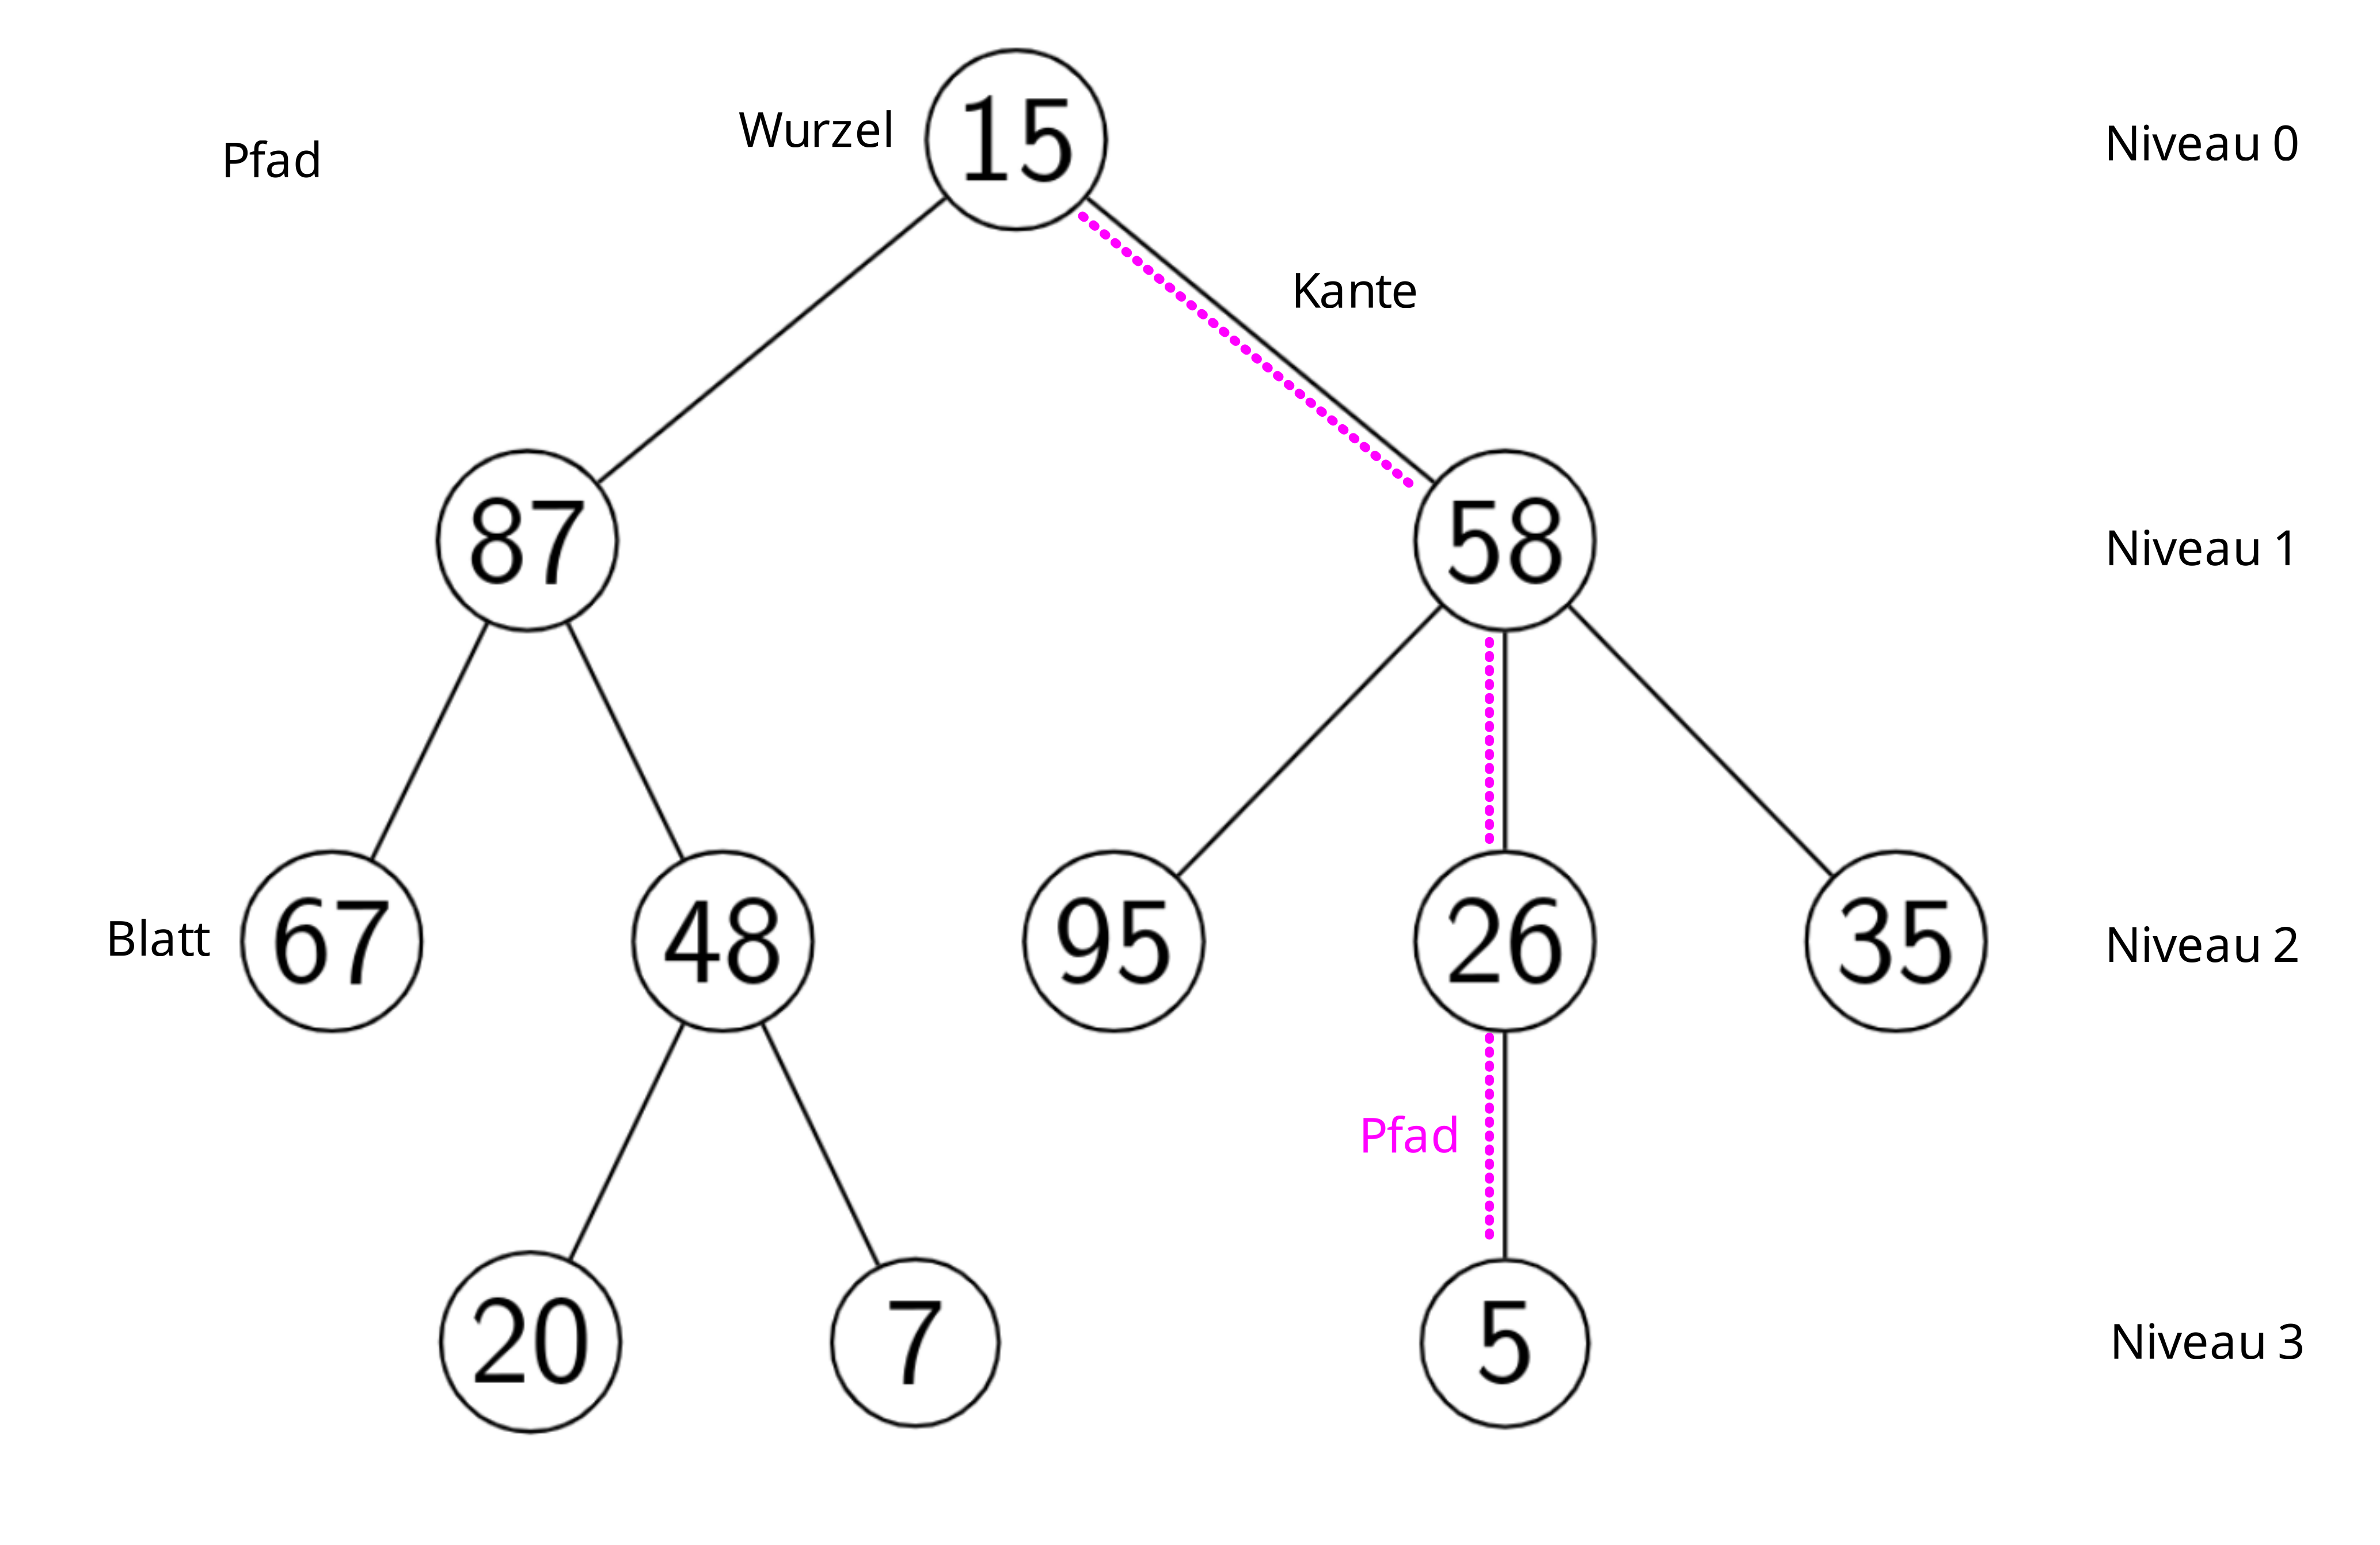
\includegraphics[width=1\textwidth]{images/baum_begriffe.png}
    \caption{\textbf{Fachbegriffe bei Bäumen}}
\end{figure}


\subsubsection{Traversierung von Binärbäumen}

Es gibt 3 gängige Verfahren zum Traversieren von Binärbaumen, um z. B. dann die Elemente
in einer anderen Datenstruktur (e.g. Schlange) zu speichern.
Alle 3 Varianten werden dabei Rekursiv beschrieben (eine Rekursive implementierung ist nicht nötig).

% tree to make images of
% \vspace*{0.3cm}

% \begin{forest}
%     for tree={
%         grow=south,
%         circle, draw, minimum size=3ex, inner sep=1pt,
%         s sep=7mm
%     }
%     [15
%         [87
%             [67]
%             [48
%                 [20]
%                 [7]
%             ]
%         ]
%         [58
%             [95]
%             [26
%                 [5]
%             ]
%             [35]
%         ]
%     ]
% \end{forest}


\subsubsection*{Pre-Order}

1. Verarbeite den Wert der Wurzel

2. Führe Pre-Order auf den linken Teilbaum aus.

3. Führe Pre-Order auf den rechten Teilbaum aus.

\vspace*{0.5cm}

\begin{forest}
for tree={
    grow=south,
    circle, draw, minimum size=3ex, inner sep=1pt,
    s sep=7mm
}
[1
    [2
        [3]
        [4]
    ]
    [5
        [6]
        [7]
    ]
]
\end{forest}

\subsubsection*{In-Order}

1. Führe In-Order auf den linken Teilbaum aus.

2. Verarbeite den Wert der Wurzel

3. Führe In-Order auf den rechten Teilbaum aus.

\vspace*{0.5cm}

\begin{forest}
for tree={
    grow=south,
    circle, draw, minimum size=3ex, inner sep=1pt,
    s sep=7mm
}
[4
    [2
        [1]
        [3]
    ]
    [6
        [5]
        [7]
    ]
]
\end{forest}

\vspace*{0.3cm}

Ist der Binärbaum sortiert, sodass z. B. für jeden Teilbaum der Wert des linken 
Unterknotens kleiner und der des rechte Unterknotens größer ist als der Wert der Wurzel,
so werden die Elemente auf- bzw. absteigend sortiert durchlaufen.

\subsubsection*{Post-Order}

1. Führe Post-Order auf den linken Teilbaum aus.

2. Führe Post-Order auf den rechten Teilbaum aus.

3. Verarbeite den Wert der Wurzel

\vspace*{0.5cm}

\begin{forest}
for tree={
    grow=south,
    circle, draw, minimum size=3ex, inner sep=1pt,
    s sep=7mm
}
[7
    [3
        [1]
        [2]
    ]
    [6
        [4]
        [5]
    ]
]
\end{forest}

\section{Rekursion}
\subsection{Fachbegriffe der Rekursion}
\subsection{Rekursionsarten}
\subsection{Divide and Conquer}
\section{Algorithmen}

\subsection{Binäre Suche}



\subsection{Quicksort}
\section{Codierung}
\subsection{Lauflängen-Codierung}
\subsection{Huffman-Codierung}
\subsection{}
\section{Objektorientierung}
\subsection{Klassen}

Die Objektorientierte Programmierung mit Klassen hat zum Ziel,
reale Zusammenhänge zu modellieren und Dinge zu strukturen und
zu organisieren. Dazu gibt es Klassen mit Attributen und Methoden
mit denen sich Objekte (Instanzen der Klasse) erzeugen lassen.
Eine Klasse ist ein Schemata zur Erzeugung eines Objekts.

\pgfsetlayers{package0, main}

\vspace*{0.5cm}
\begin{figure}[H]
\begin{center}
\hspace*{-2cm}
\begin{minipage}{.7\textwidth}
    \begin{lstlisting}[language=python]
    class Car:
        def __init__(self, name: str, speed: float):
            self.name = name      # Attribut
            self.speed = speed
            self.__km_driven = 0
            
        def getDriven() -> float: # Methode
            return self.__km_driven
            
        def drive(hours: float):
            self.__km_driven += self.speed * hours
    \end{lstlisting}
    \caption{Klasse Auto in Python}
\end{minipage}
\begin{minipage}{.3\textwidth}
    \begin{tikzpicture}
        \umlclass{Auto}{ 
        + name : Zeichenkette \\ 
        + speed : Dezimalzahl \\ 
        - km\_driven : Dezimalzahl
        }{ 
            + getDriven() : Dezimalzahl \\
            + drive(hours: Dezimalzahl) :
            }
    \end{tikzpicture}
    \caption{UML Klassendiagramm}
\end{minipage}
\end{center}
\end{figure}

\subsection{Vererbung}

Bei der Vererbung wird eine Klasse auf Basis einer anderen Definiert.
Diese Unterklasse übernimmt dann alle Attribute und Methoden der Oberklasse
und kann noch weitere hinzufügen oder neu definieren. Vererbung lässt sich auch
Verketten. Klasse A erbt von B und Klasse B erbt von C. So hat A auch die Attribute
und Methoden von C.

\pgfsetlayers{package0, main, connections}

\vspace*{0.5cm}
\begin{figure}[H]
\begin{center}
    \begin{tikzpicture}
        \umlclass[x=-4,]{Auto}{ 
            + name : Zeichenkette \\ 
            + speed : Dezimalzahl \\ 
            - km\_driven : Dezimalzahl
        }{ 
            + getDriven() : Dezimalzahl \\
            + drive(hours: Dezimalzahl) :
        }
        \umlclass[x=4, y=-1]{Mercedes}{ 
            + preis : Ganzahl \\
            + topspeed: Dezimalzahl
        }{
            + speedPerPrice() : Dezimalzahl\\
        }
        \umlinherit{Mercedes}{Auto}
    \end{tikzpicture}
    \caption{Vererbung}
\end{center}
\end{figure}

\begin{figure}
\begin{lstlisting}[language=python]
class Mercedes(Auto): # Vererbung
    def __init__self(self, name: str, speed: float, preis: Ganzahl, topspeed: Dezimalzahl):
        self.name = name      # geerbtes Attribut
        self.speed = speed    # geerbtes Attribut
        self.__km_driven = 0  # geerbtes Attribut
        self.preis = preis
        self.topspeed = topspeed

    def speedPerPrice() -> float: # neue Methode
        return self.topspeed / self.preis
\end{lstlisting}
\caption{Klasse Mercedes in Python}
\end{figure}

\subsection{Klassendiagramme}

Die Unified Modeling Language (UML) kann für sogenannte UML-Diagramme zur abstrakten
Modellierung genutzt werden (von der Programmiersprache unabhängig).
Im oberen Teil einer Klasse werden die Attribute mit Datentyp definiert.
Im unteren Teil werden die Methoden der Klasse mit Rückgabewert definiert.
Ein Plus bedeutet öffentlich, ein Minus bedeutet Privat, ein Hashtag
bedeutet Geschützt und eine Tilde bedeutet nur im Package sichtbar.
Eine Vererbung wird durch einen Pfeil mit unausgefülltem Ende von der erbenden
zur vererbenden Klasse dargestellt. Eine Assoziation ist einfach eine Linie.

\vspace*{0.5cm}
\begin{figure}[H]
\begin{center}
    \begin{tikzpicture}
        \umlclass[x=-2,y=5]{Autohaus}{ 
            + autos : Reihung vom Typ Auto \\ 
        }{ 
            + getAutoCount() : Ganzzahl \\
        }
        \umlclass[x=-4,]{Auto}{ 
            + name : Zeichenkette \\ 
            + speed : Dezimalzahl \\ 
            - km\_driven : Dezimalzahl
        }{ 
            + getDriven() : Dezimalzahl \\
            + drive(hours: Dezimalzahl) :
        }
        \umlclass[x=4, y=-1]{Mercedes}{ 
            + preis : Ganzahl \\
            + topspeed: Dezimalzahl
        }{
            + speedPerPrice() : Dezimalzahl\\
        }
        \umlassoc{Auto}{Autohaus}
        \umlinherit{Mercedes}{Auto}
    \end{tikzpicture}
    \caption{Klassendiagramme}
\end{center}
\end{figure}


\section{Datenbanken}

\subsection{Begriffe bei Datenbanken}

In relationnellen Datenbanksystemen werden Daten als Entitäten modelliert
und strukturiert in sogenannten Tabellen (Relationen) gespeichert. Zwischen
diesen Tabellen werden dann auch zusammenhänge modelliert.

\vspace*{0.3cm}

Tabellen bestehen aus Zeilen (Datensätzen) und Spalten. Jede Spalte
steht dabei für ein Attribut der Tabelle, sodass jeder Datensatz
einen passenden Wert für jedes Attribut der Tabelle, also für jede Spalte, haben
muss. Jede Tabelle definiert ein oder mehrere Attribute, die den Primärschlüssel
darstellen. Der Primärschlüssels darf in keinen Datensätzen gleich sein, da dieser
zur eindeutigen Identifikation eines Datensatzes genutzt wird.
Außerdem gibt es noch Fremdschlüssel, die in Attributen einer Tabelle
gespeichert werden können. Dies sind Primärschlüssel einer anderen Tabelle,
wodurch Zusammenhänge zwischen Tabellen hergestellt werden können.

\vspace*{0.3cm}

Datensatz: Grau

Primärschlüssel: Blau

Attribut: Rot

Fremdschlüssel: Gelb

\begin{table}[H]
    \begin{tabular}{|l|l|l|}
    \hline
        CD\_ID & Albumtitel & Interpret\_ID \\ \hline
        \rowcolor{gray!20} 11 & Los Angeles & 21 \\ \hline
        12 & Goodbye New York & 22 \\ \hline
        13 & Dr. Drug & 21 \\ \hline
    \end{tabular}
\end{table}

\begin{table}[H]
    \begin{tabular}{|>{\columncolor{blue!20}}l|>{\columncolor{red!20}}l|>{\columncolor{yellow!50}}l|}
    \hline
        CD\_ID & Albumtitel & Interpret\_ID \\ \hline
        11 & Los Angeles & 21 \\ \hline
        12 & Goodbye New York & 22 \\ \hline
        13 & Dr. Drug & 21 \\ \hline
    \end{tabular}
\end{table}

\clearpage

\subsection{Entity-Relationship-Modelle (ER-Modelle)}

Ein Entity-Relationsip Modell soll Entitäten und Beziehungen eines Sachverhalts
darstellen und so z. B. die Erstellung einer Datenbank erleichtern.
Es gibt mehrere Arten zur Notation von Entity Relationship Modellen,
in diesem Fall wird die Chen Notation betrachtet.

\vspace*{1cm}

\adjustbox{scale=0.8}{
\begin{tikzpicture}[auto,node distance=1cm]
\node[entity] (node1) {Student}[grow=up,sibling distance=3.5cm]
    child[text width=2cm, align=center, level distance=2cm] {node[attribute] {Lastname}}
    child[text width=2cm, align=center, level distance=2cm] {node[attribute] {Firstname}}
    child[text width=2cm, align=center, level distance=2cm] {node[attribute] {\underline{ID}}};

\node[relationship] (rel1) [below = of node1] {Takes};
\node[attribute] (node4) [left = of rel1] {Hours};
\path (rel1) edge (node4);

\node[entity] (node2) [below = of rel1]{Class}[grow=down,sibling distance=3.5cm]
    child[text width=2cm, align=center, level distance=2cm] {node[attribute] {\underline{ID}}}
    child[text width=2cm, align=center, level distance=2cm] {node[attribute] {Subject}}
    child[text width=2cm, align=center, level distance=2cm] {node[attribute] {Teacher}};
\path (rel1) edge node {n} (node1) edge node {m}(node2);

\node[relationship] (rel2) [right = of node1] {Goes To};

\node[entity] (node3) [right = of rel2]{School}[grow=right, sibling distance=2.5cm]
    child[text width=2cm, align=center, level distance=2cm] {node[attribute] {\underline{ID}}}
    child[text width=2cm, align=center, level distance=2cm, xshift=2cm] {node[attribute] {Name}}
    child[text width=2cm, align=center, level distance=2cm] {node[attribute] {Type}};

\path (rel2) edge node {m} (node1) edge node {1}(node3);
\end{tikzpicture}
}

\vspace*{0.3cm}

\subsubsection{Erklärung der ER-Notation nach Chen}

\vspace*{0.3cm}

\begin{enumerate}
    \item Ein Rechteck stellt eine Entität dar.
    \item Ein Oval stellt ein Attribut einer Entität dar.
    \item Ein unterstrichenes Attribut ist Teil des Primärschlüssels.
    \item Eine Raute erläutert die Beziehung zweier Entitäten.
    \item Ein Oval an einer Raute kann der Beziehung Attribute zuordnen.
    \item An einer Beziehung zwischen zwei Entitäten sind die Kardinalitäten notiert.
\end{enumerate}

\clearpage

\subsubsection{Kardinalitäten}

Die Kardinälität einer Beziehung beschreibt, wie vielen Entitäten der anderen
Entität zugeordnet werden können. Beispielsweise kann ein Schüler nur auf 1 Schule 
gehen, aber auf eine Schule können viele Schüler gehen. Klassen besucht ein Schüler
hingegen mehrere und in eine Klasse gehen mehrere Schüler. Es gibt folgende Kardinalitäten,
wobei man bei jeder Kardinalität auch angeben kann, ob einer Zuordnung optional ist
oder wie viele Zuordnung es geben muss.

\begin{table}[H]
    \begin{tabular}{|l|l|l|}
    \hline
        Kardinälität & Entität A & Entität B \\ \hline
        Eins zu Eins & 1 & 1 \\ \hline
        Eins zu Vielen & 1 & m \\ \hline
        Viele zu Eins & m & 1 \\ \hline
        Viele zu Viele & m & n \\ \hline
        \end{tabular}
\end{table}

\subsection{Normalformen}

Bei der Erstellung eines Datenbankschemas in einer Relationellen Datenbank
(z. b. aus einem ER-Modell) unterscheidet man, je nach Eigentschaften des
Schematas, in welcher Normalform sich dieses befindet. Ein Schemata kann
von einer Normalform in eine andere (nächthöhere) überführt werden.
Dies lässt sich auch automatisiert durchführen. Jede dieser Normalformen
unterscheidet sich darin, wie die Abhängigkeiten zwischen den Tabellen
und Attributen sind. Je höher die Normalform, desto weniger Redundanz der Daten
(Wiederholung) ist vorhanden und desto weniger Inkosistenz und Anomalien gibt es.

\subsubsection{0. Normalform}

Die Daten liegen unstrukturiert, redundant und nicht-atomar vor.

\newcolumntype{a}{>{\columncolor{blue!20}}l}
\newcolumntype{d}{>{\columncolor{yellow!50}}l}

\begin{table}[H]
    \begin{tabular}{|a|l|l|l|}
    \hline
        CD\_ID & Albumtitel & Gründungsjahr & Titelliste \\ \hline
        11 & Sniff Dog - Los Angeles & 1995 & {1. Crazy 2. Love 3. Crack} \\ \hline
        12 & Jay-X - Goodbye New York & 1965 & {1. Imperial State of Math} \\ \hline
        13 & Sniff Dog - Dr. Drug & 1999 & {1. Weed Every Day} \\ \hline
    \end{tabular}
\end{table}

\clearpage

\subsubsection{1. Normalform}

Die Anforderungen an die 1. NF sind, dass alle Attribute atomar sind und
unnötige Spalten und Daten zusammengefasst werden, ohne das Informationen verloren gehen.

\begin{table}[H]
    \begin{tabular}{|a|l|l|l|a|l|}
    \hline
        CD\_ID & Albumtitel & Interpret & Gründungsjahr & Track & Titelliste \\ \hline
        11 & Los Angeles & Sniff Dog & 1993 & 1 & Crazy \\ \hline
        11 & Los Angeles & Sniff Dog & 1993 & 2 & Love \\ \hline
        11 & Los Angeles & Sniff Dog & 1993 & 3 & Crack \\ \hline
        12 & Goodbye New York & Jay-X & 1965 & 1 & Imperial State of Math \\ \hline
        13 & Dr. Drug & Sniff Dog & 1993 & 1 & Weed Every Day \\ \hline
    \end{tabular}
\end{table}

\subsubsection{2. Normalform}

Die Anforderungen an die 2. NF sind die an alle Vorigen und dass keine
nicht-schlüssel Attribute in einer Relation nur von einem Teil des Primärschlüssels
abhängig sind (jedes Attribut einer Relation ist voll funktional abhängig vom Primärschlüssel dieser).

\begin{table}[H]
    \begin{tabular}{|a|l|l|l|}
    \hline
        CD\_ID & Albumtitel & Interpret & Gründungsjahr \\ \hline
        11 & Los Angeles & Sniff Dog & 1993 \\ \hline
        12 & Goodbye New York & Jay-X & 1965 \\ \hline
        13 & Dr. Drug & Sniff Dog & 1993 \\ \hline
    \end{tabular}
\end{table}

\begin{table}[H]
    \begin{tabular}{|a|a|l|}
    \hline
        CD\_ID & Track & Titel \\ \hline
        11 & 1 & Crazy \\ \hline
        11 & 2 & Love \\ \hline
        11 & 3 & Crack \\ \hline
        12 & 1 & Imperial State of Math \\ \hline
        13 & 1 & Weed Every Day \\ \hline
    \end{tabular}
\end{table}

\clearpage

\subsubsection{3. Normalform}

Die Anforderungen an die 3. NF sind die an alle Vorigen und dass keine
nicht-schlüssel Attribute in einer Relation von anderen nicht-schlüssel Attributen
funktional abhängegen. Diese nicht gewollten Abhängigkeiten nennt man transistive Abhängigkeiten.

\begin{table}[H]
    \begin{tabular}{|a|l|d|}
    \hline
        CD\_ID & Albumtitel & Interpret\_ID \\ \hline
        11 & Los Angeles & 21 \\ \hline
        12 & Goodbye New York & 22 \\ \hline
        13 & Dr. Drug & 21 \\ \hline
    \end{tabular}
\end{table}

\begin{table}[H]
    \begin{tabular}{|a|l|l|}
    \hline
        Interpret\_ID & Interpret & Gründungsjahr \\ \hline
        21 & Sniff Dog & 1993 \\ \hline
        22 & Jay-X & 1965 \\ \hline
        21 & Sniff Dog & 1993 \\ \hline
    \end{tabular}
\end{table}

\begin{table}[H]
    \begin{tabular}{|a|a|l|}
    \hline
        CD\_ID & Track & Titel \\ \hline
        11 & 1 & Crazy \\ \hline
        11 & 2 & Love \\ \hline
        11 & 3 & Crack \\ \hline
        12 & 1 & Imperial State of Math \\ \hline
        13 & 1 & Weed Every Day \\ \hline
    \end{tabular}
\end{table}

\clearpage

\subsection{Datenbanken Anomalien und Inkonsistenz}

Es gibt 3 Arten von Anomlien in Datenbanken. Einfüge-, Änderungs- und Löschanomlie.
Diese treten meist auf, wenn das Datenbankschema unklar oder schlecht ist und Redundanzen
aufweist. Dies führt zur Inkonsistenz der Datenbank. Das heißt, es fehlen wichtige
Daten oder es gibt konfliktierende Datensätze, was die Integrität der Datenbank mindert.

\subsubsection{Einfügeanomlie}

Eine Einfügeanomalie tritt dann auf, wenn beim Einfügen eines Datensatzes
nicht alle Spalten mit einem Wert gefüllt werden können, z. B. weil der
Wert aufgrund des Sachzusammenhangs noch nicht bekannt ist.
Dadurch entstehen inkonsistenzen.
Beispielsweise hat ein Künstler sich noch nicht für einen Songnamen entschieden.

\begin{table}[H]
    \begin{tabular}{|a|a|l|}
    \hline
        CD\_ID & Track & Titel \\ \hline
        11 & 1 & Crazy \\ \hline
        11 & 2 & Love \\ \hline
        11 & 3 &  \\ \hline
        \end{tabular}
\end{table}

\subsubsection{Änderungsanomalie}

Ein Änderungsanomlie tritt dann auf, wenn Daten redundant vorliegen und bei
der Änderung z. B. eines Attributs nicht alle anderen Einträge auch geändert
werden. Dadurch gibt es konflikte der Daten, also Inkonsistenz.
Wird Beispielsweise der Albumname nicht für alle Songs geändert,
so weiß man nicht, welcher Name der Richtige ist.

\begin{table}[H]
    \begin{tabular}{|a|a|l|l|}
    \hline
        CD\_ID & Track & Albumtitel & Titel \\ \hline
        11 & 1 & Crazy & Los Angeles \\ \hline
        11 & 2 & Love  & Los Angeles\\ \hline
        11 & 3 & Crack & San Francisco \\ \hline
        \end{tabular}
\end{table}

\subsubsection{Löschanomlie}

Bei der Löschanomlie werden ungewollt Daten gelöscht. Dies
geschieht z. B. dann, wenn Beziehungen nicht in seperaten
Tabellen gespeichert sind oder wenn die Tabellen nicht korrekt
aufgebaut sind.

\clearpage

\subsection{SQL}

Das Aufsetzen eines Datenbank Servers und einer Datenbank sowie das Erstellen und
Modifizieren von Tabellen und die Grundlegenden Datentypen werden im folgenden
nicht behandelt. Es wird ein Fokus auf SQL-Abfragen gelegt.

\subsubsection{Strukturübersicht von SQL Abfragen}

<TODO: erklärung>

\adjustbox{scale=1.3}{
\begin{lstlisting}
Abfragestruktur:
SELECT [DISTINCT | ALL] columns FROM tables
[WHERE bedingung1 (AND | OR) bedingung2 (AND | OR) ...]
[GROUP BY spalte1 , spalte2 , ...]
[HAVING bedingung1 (AND | OR) bedingung2 (AND | OR) ...]
[ORDER BY spalte1 [ASC | DESC], spalte2 [ASC | DESC], ...]
[LIMIT anzahl]

Operatoren für Berechnungen:
+, -, *, /

Operatoren für Vergleiche in Bedingungen: 
=, != , >, <, >=, <=, NOT
LIKE (mit den Platzhaltern _ und %) , BETWEEN, IN, IS NULL

Aggregatfunktionen: AVG( ), COUNT( ), MAX( ), MIN( ), SUM( ) 
\end{lstlisting}
}

\section{Kryptologie}
\subsection{Verschlüsselung im Alltag}

Verschlüsselung ist ein Grundpfeiler der modernen Kommunikation und absolut nötig,
damit kein Unbekannter und Unbefugter private Nachrichten oder Passwörter mitlesen
kann. Ohne starke Verschlüsselungsverfahren, wäre die weitergabe sensibler Daten über
das Internet nicht möglich.

\subsection{Historische Verschlüsselungsverfahren}

\subsubsection{Caesar Chiffre}

Schon die alten Römer und viele nach ihnen erkannten, dass es durchaus von Vorteil
ist, wenn die Feinde nichts über den geheimen Schlachtplan oder die nächste Intrige
erfahren können.
Das sogenannte Caesar-Chiffre ist die einfachste Form eines symetrischen,
monoalphatischen Verschlüsselungsverfahren für Texte.
Man bestimmt eine Verschiebung zwischen 1 und 25 und ersetzt dann
alle Buchstaben des Klartexts, um den Geheimtext zu erhalten.
Kennt man die Verschiebung, so lässt sich die Nachricht auch wieder entschlüsseln.
Dieses Verfahren ist allerdings nicht sicher, weswegen es heutzutage niemand verwendet.
Um einen Buchstaben zu verschlüsseln sucht man diesen im oberen Alphabet und
ersetzt diesen dann durch den Buchstaben darunter aus dem unteren Alphabet.
Beim Entschlüsseln ist dies umgekehrt. Man ersetzt den Buchstaben im Geheimtext
durch den Buchstaben aus dem oberen Alphabet, der über der Position des Buchstabens
im unteren Alphabet ist.

\begin{lstlisting}
A B C D E F G H I J K L M N O P Q R S T U V W X Y Z
Y Z A B C D E F G H I J K L M N O P Q R S T U V W X

Klartext:     INFORMATIK
Geheimtext: GLDMPKYRGI
\end{lstlisting}

\clearpage

\subsection{Symetrische Verschlüsselung}

Symetrische Verschlüsselungsverfahren zeichnen sich dadurch aus, dass zum
Ent- und Verschlüsseln der gleiche Algorithmus und der gleiche Schlüssel verwendet
wird. Beispiele sind die Caesar Chiffre, die Vigenere Chriffe oder das Blockchiffre AES-256.

\subsubsection{Blockchriffen}

Blockchiffre Verfahren sind symetrische Verschlüsselungsverfahren,
die auch zur Verschlüsselung größerer Datenmengen genutzt werden können.
Eine besondert dieser ist, dass die zu verschlüsselnden Daten Blockweise
verschlüsselt werden und in die Verschlüsselung eines Block ein Ergebnis
der Verschlüsselung des vorigen Blocks mit eingeht.
Blockchiffren wie Advanced Encryption Standard (AES) mit hohen Bitlängen (e.g. AES-256)
sind mit heutigen Mitteln unknackbare Verfahren, weswegen dies breite Anwendung
z. B. bei Datenübertragung oder Festplattenverschlüsselung finden.

\subsubsection{Diffie-Hellman Verfahren}

Dieses von Whitfield Diffie und Martin Hellman entwickelte Verfahren ermöglicht es,
dass zwei Kommunikationspartner einen gemeinsamen, geheimen Schlüssel in Form einer Zahl
vereinbaren, auch wenn ihre Kommunikationsleitung öffentlich (unverschlüsselt ist).
Dadurch lassen sich einfach Schlüssel austauschen, um danach z. B. die Kommunikation
mit AES zu verschlüsseln.

\begin{lstlisting}
a: 0 < natürliche Zahl < p
b: 0 < natürliche Zahl < p
p: öffentliche Primzahl
g: 0 < öffentliche natürliche Zahl < p
A: öffentliche Schlüssel Alice
B: öffentliche Schlüssel Bob
K: geheimer Schlüssel, nur Bob und Alice bekannt
\end{lstlisting}

\begin{figure}[H]
    \centering
    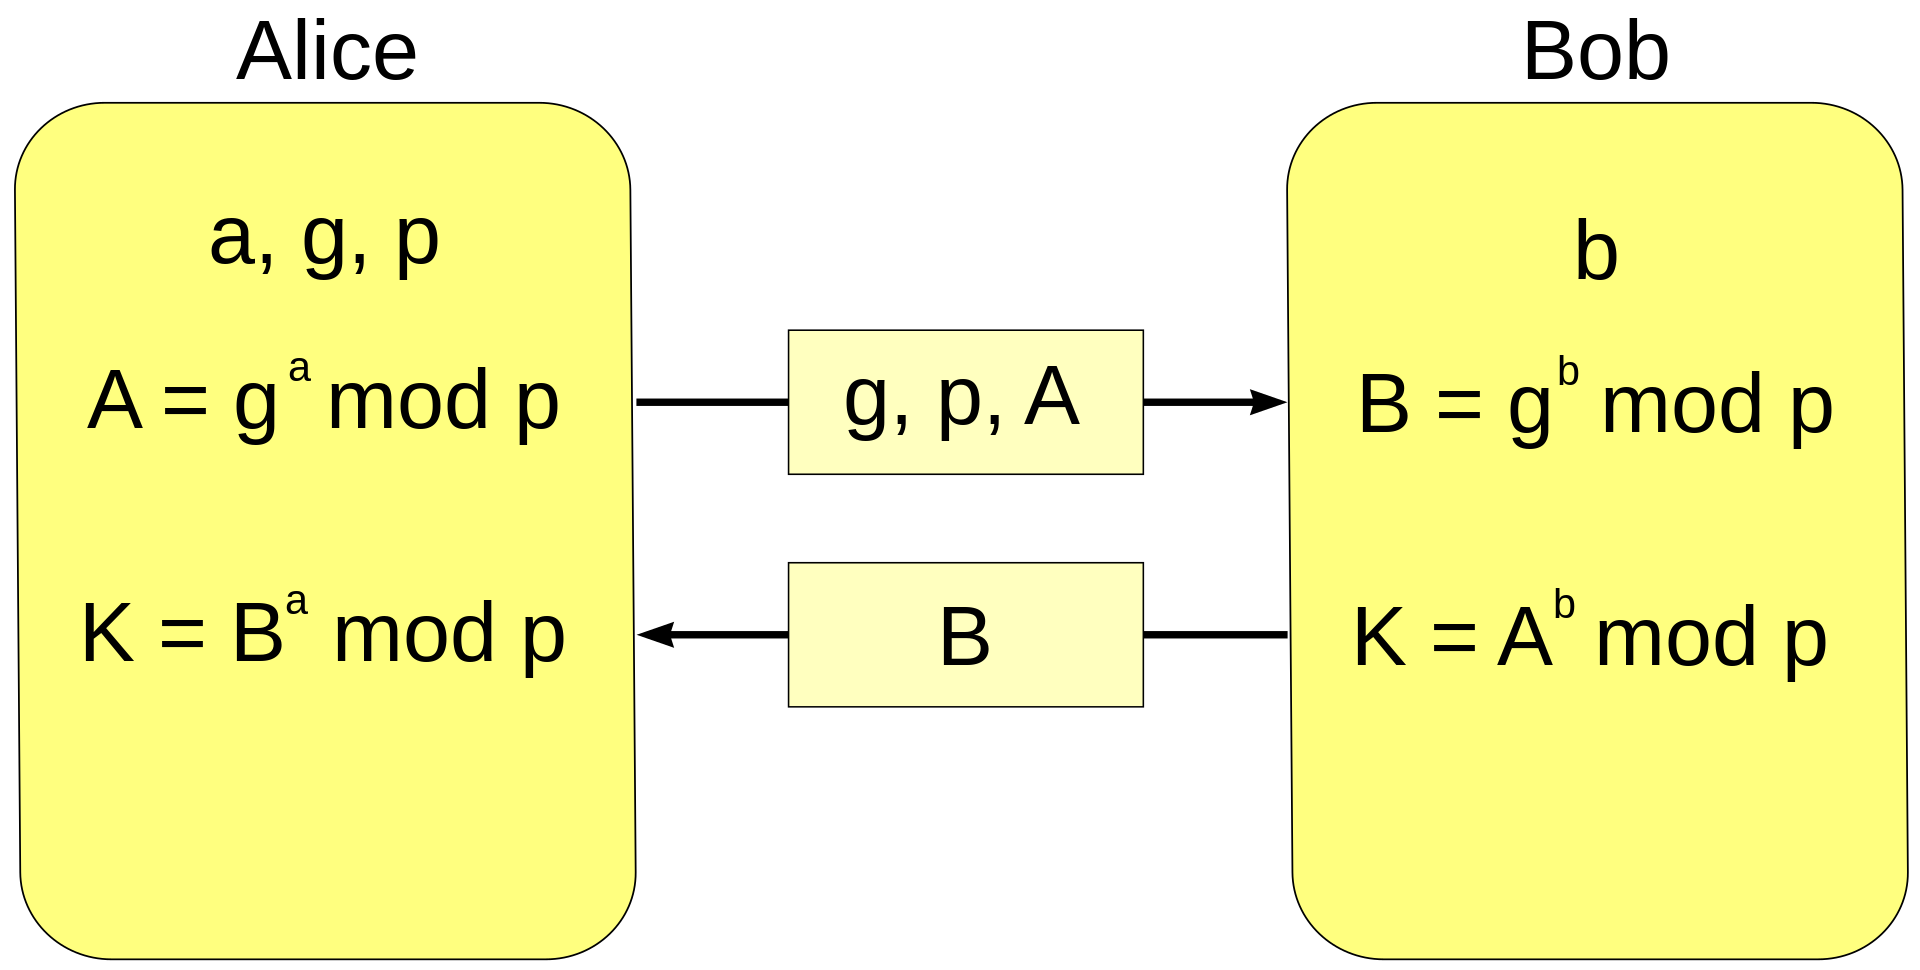
\includegraphics[width=0.6\textwidth]{images/diffie-hellman.png}
    \caption{Diffie-Hellman Schlüsseltausch}
\end{figure}

\clearpage

\subsection{Asymetrische Verschlüsselung (Public Key Cryptography)}

Die asymetrische Verschlüsselung zeichnet sich im Unterschied zur symetrischen
Verschlüsselung dadurch aus, dass es 2 Schlüssel gibt. Den einen zum Ver-, den anderen
zum Entschlüsseln. Diese beiden Schlüssel nennt man ein Schlüsselpaar.

\subsubsection{Schlüsselpaare}
Es gibt verschiedene Algorithmen, um kryptographische Schlüsselpaare zu erstellen.
Die bekanntesten und besten sind RSA und EdDSA und Variationen dieser.
Je nach Verfahren kann die Bitlänge der Schlüssel variieren, wobei höhere Bitlängen
sicherer sind. Die eigenschaften des Schlüsselpaars sind wie folgt.

\begin{lstlisting}
privater Schlüssel (öffentlicher Schlüssel (Nachricht)) = Nachricht
öffentlicher Schlüssel (privater Schlüssel (Nachricht)) = Nachricht 
\end{lstlisting}

\subsubsection{Verschlüsselung mit Public und Private Key}

Beide Kommunikationspartner erstellen ein asymetrisches Schlüsselpaar.
Anschließend übertragen beide den öffentlichen Schlüssel an den Kommunikationspartner.
Nun können Nachrichten mit dem öffentlichen Schlüssel des Partners verschüsselt werden
und nur dieser kann diese mit dem privaten Schlüssel entschlüsseln. Niemand sonst kann
so die Kommunikation mitverfolgen. Es ist auch möglich, nun einen symetrischen Schlüssel
auszutauschen und z. B. AES-256 in der weiteren Kommunikation zu verwenden.

\begin{figure}[H]
    \centering
    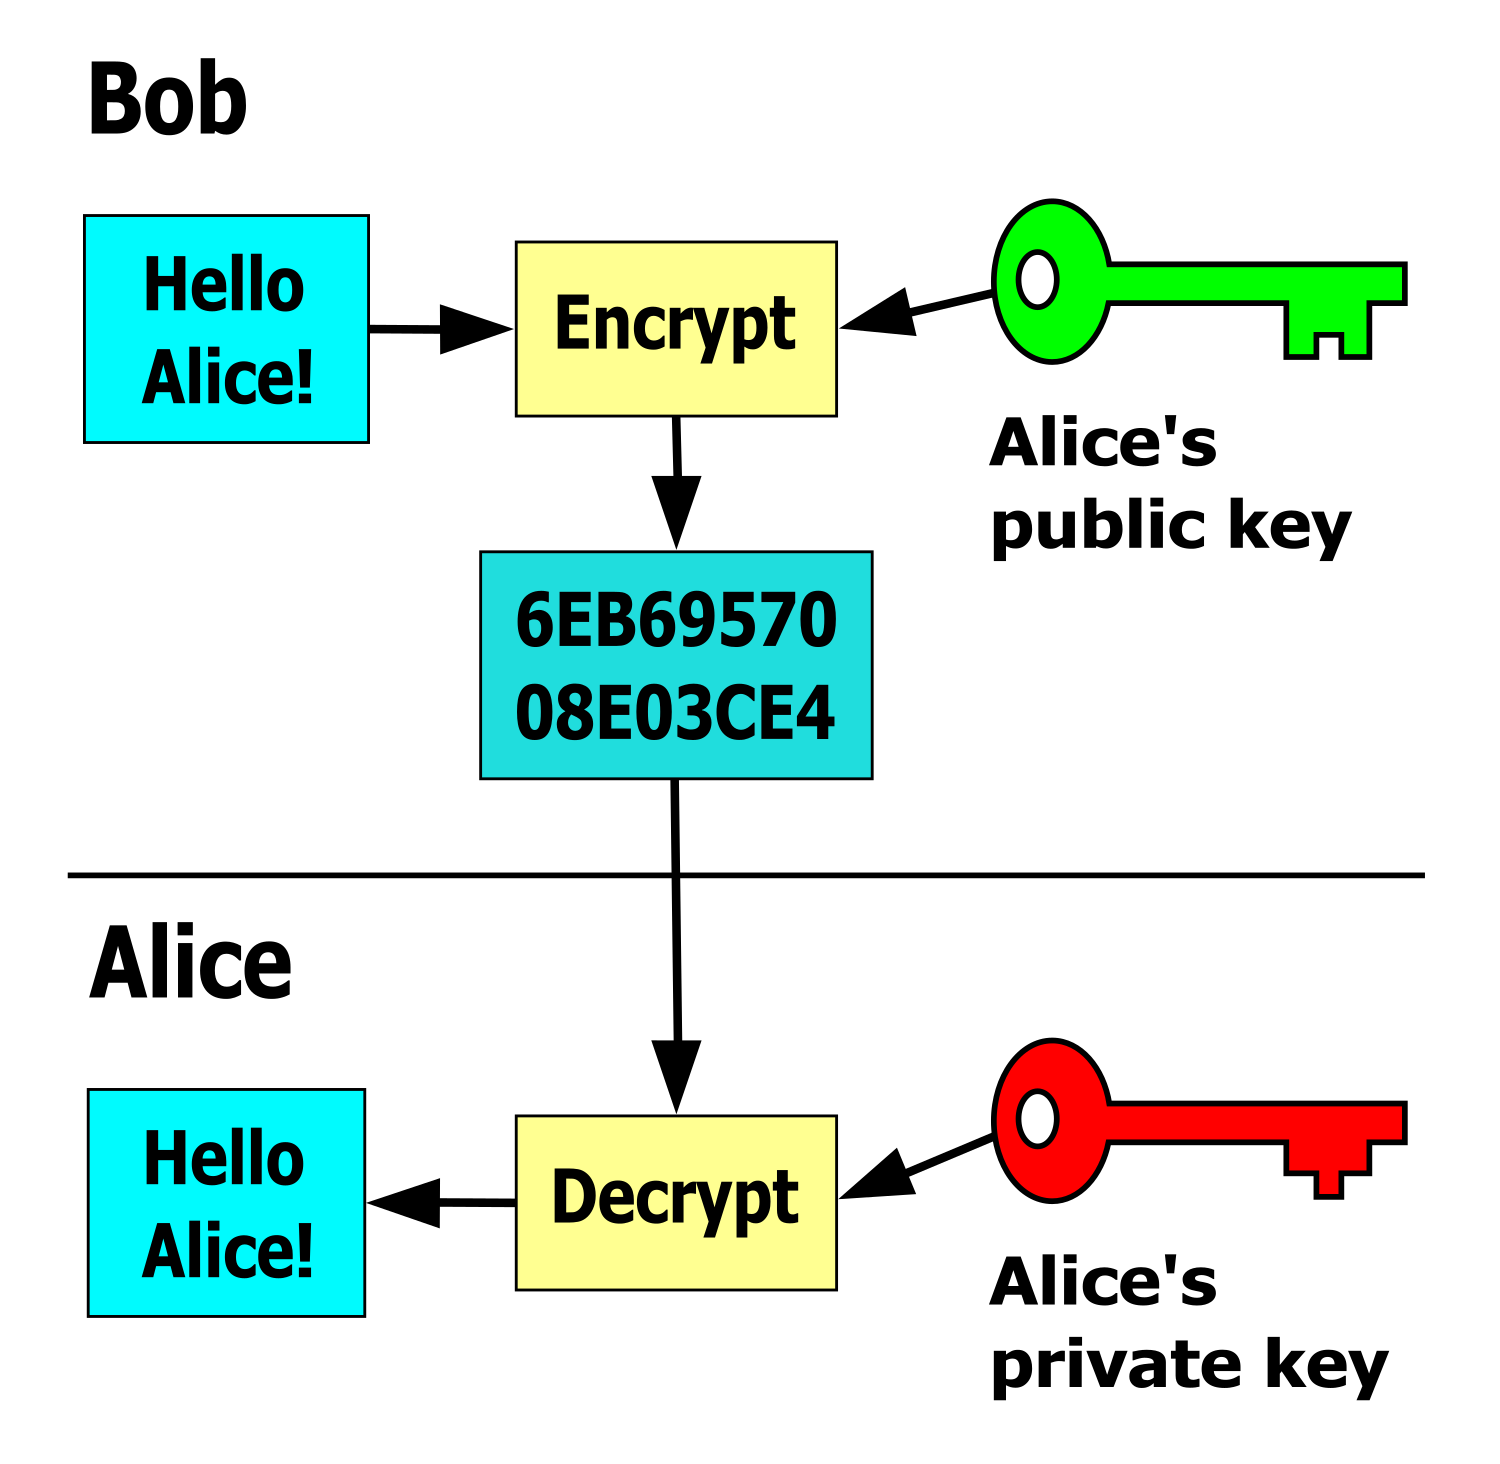
\includegraphics[width=0.5\textwidth]{images/public-key-encryption.png}
    \caption{Verschlüsselung mit Schlüsselpaaren}
\end{figure}

\clearpage

\subsection{Digitale Signaturen}

\subsubsection{Das Authentizitätsproblem}

Wenn Alice und Bob ihre Schlüssel ausgetauscht haben, kann niemand ihre Nachrichten mitlesen.
Doch fängt jemand jeweils die öffentlichen Schlüssel von Bob und Alice bei der Übertragung ab,
so kann diese Person Beiden Nachrichten schicken, von denen diese denken, sie wärem vom
jeweils anderen.

\subsubsection{Lösung mit digitalen Signaturen und Hash-Werten}

Damit Alice und Bob sicher sein können, dass niemand ihre Nachrichten verändert oder
ihnen Falschnachrichten sendet, können diese ihre Nachrichten mit ihren Schlüsseln signieren.
Anstatt ihre Nachricht nur mit Bobs öffentlichem Schlüssel zu verschlüsseln, wendet Alice vorher noch
ihren Privaten Schlüssel auf die Nachricht an. Jede Person mit Alice öffentlichem Schlüssel
kann so feststellen, dass die Nachricht von ihr kommt. Würde man diese Nachricht mit Alice
öffentlichem Schlüssel entschlüsseln wollen, und es wäre ein anderer privater Schlüssel
verwendet worden (z. B. von Eve), so würde sich keine Nachricht ergeben und man wüsste,
dass diese Nachricht nicht von Alice sein kann. Anschließend verschlüsselt sie wie vorher
auch die Nachricht mit Bob öffentlichem Schlüssel, da diese sonst jeder mitlesen könnte.
Nur Bob kann nun die Nachricht entschlüsseln und anschließend kann er mit Alice öffentlichem
Schlüssel die Authentizität überprüfen. Nun kann niemand anderes Bob Nachrichten in Alice Namen
senden. Gleiches gilt nun natürlich auch für Alice.

\begin{lstlisting}[basicstyle=\small]
PubKeyBob (PrivKeyAlice (Alice Nachricht)) = Alice Nachricht verschlüsselt und signiert
PrivKeyBob (Alice Nachricht verschlüsselt und signiert) = Alice Nachricht signiert
PubKeyAlice (Alice Nachricht signiert) = Nachricht
\end{lstlisting}

Ist Alice Nachricht sehr groß und sie will nicht auf die komplette Nachricht
ihren privaten Schlüssel anwenden (z. B. aus Effizienzgründen), so kann sie
einen Hash-Wert (diese ist deutlich kürzer als die Nachricht) der Nachricht erstellen
und nur diesen signieren. Anschließend verschlüsselt sie dann die Nachricht und
den signierten Hash-Wert und schickt diese an Bob.
Bob weiß, dass nur Alice ihm diesen Hash-Wert übermittelt haben kann, und kann so
prüfen, ob der Hash-Wert zur Nachricht passt, also ob die Nachricht wirklich von Alice
ist. Dazu nutzt er die gleiche Hash-Funktion wie Alice und prüft, ob sein und der signierte
Hash-Wert der gleiche sind.

\subsubsection{Erklärung von Hash-Funktionen und Hash-Werten}

Eine Hash-Funktion erstellt zu einer Eingabe an Daten einen Hash-Wert fester Länge.
Für die gleichen Daten ist dieser Hash-Wert beim mehrmaligen ausführen der 
Funktion auf diese Daten immer gleich.
Bei einer guten, kryptographisch sicheren Hash-Funktionen haben nahezu nie verschiedene
Daten den gleichen Hash-Wert und eine Umkehr der Funktion ist nicht einfach möglich.
Dadurch wird verhindert, dass man zu einem Hash-Wert einfach die Daten finden kann, die
diesen erzeugen.

\subsection{Zertifikate}

\subsubsection{Das Integritätsproblem}

Jetzt schaltet sich jedoch Eve dazwischen und startet einen Man-in-the-Middle Angriff.
Sie fängt die öffentlichen Schlüssel von Bob und Alice bei der Übertragung
ab und ersetzt diese durch einen öffentlichen Schlüssel eines anderen Schlüsselpaars (links).
Da Eve dazwischen geschaltet ist, kann sie jede Nachricht nun abfangen, entschlüsseln, lesen
und verändern (rechts). Anschließend sendet sie die Nachricht mit dem abgefangenen, echten öffentlichen
Schlüssel weiter an Bob bzw. Alice. Auch eine digitale Signatur von Alice auf die ganze Nachricht bringt nichts,
da Eve diese entschlüsseln kann und dann mit ihrem privaten Schlüssel eine neue
Signatur für Bob erstellt.

\vspace*{0.5cm}

\begin{center}
\adjustbox{scale=1.0}{
\begin{tikzpicture}
% left %
% alice
\draw (0,0) rectangle (4,2);
\node[draw] at (2,1.5) {Alice};
\node[draw=red, thick, rounded corners, fill=red!20] at (1,0.7) {Pub};
\node[draw=red, thick, rounded corners, fill=red!20] at (3,0.7) {Priv};
% eve
\draw (0,4) rectangle (4,6);
\node[draw] at (2,5.5) {Eve};
\node[draw=violet, thick, rounded corners, fill=violet!20] at (1,4.7) {Pub};
\node[draw=violet, thick, rounded corners, fill=violet!20] at (3,4.7) {Priv};
% bob
\draw (0,8) rectangle (4,10);
\node[draw] at (2,9.5) {Bob};
\node[draw=green, thick, rounded corners, fill=green!20] at (1,8.7) {Pub};
\node[draw=green, thick, rounded corners, fill=green!20] at (3,8.7) {Priv};
% arrows
\draw [-{Latex[length=2mm]}] (1,4) -- (1,2);
\draw [-{Latex[length=2mm]}] (3,2) -- (3,4);
\draw [-{Latex[length=2mm]}] (1,8) -- (1,6);
\draw [-{Latex[length=2mm]}] (3,6) -- (3,8);
% labels
\node[draw=red, thick, rounded corners, fill=red!20] at (3,3) {Pub};
\node[draw=violet, thick, rounded corners, fill=violet!20] at (1,3) {Pub};
\node[draw=violet, thick, rounded corners, fill=violet!20] at (3,7) {Pub};
\node[draw=green, thick, rounded corners, fill=green!20] at (1,7) {Pub};

% right %
% alice
\draw (6,0) rectangle (10,2);
\node[draw] at (8,1.5) {Alice};
\node[draw=red, thick, rounded corners, fill=red!20] at (7,0.7) {Priv};
\node[draw=violet, thick, rounded corners, fill=violet!20] at (9,0.7) {Pub};
% eve
\draw (6,4) rectangle (10,6);
\node[draw] at (8,5.5) {Eve};
\node[draw=red, thick, rounded corners, fill=red!20] at (6.8,4.6) {Pub};
\node[draw=violet, thick, rounded corners, fill=violet!20] at (6.8,5.4) {Priv};
\node[draw=violet, thick, rounded corners, fill=violet!20] at (9.2,4.6) {Priv};
\node[draw=green, thick, rounded corners, fill=green!20] at (9.2,5.4) {Pub};
% bob
\draw (6,8) rectangle (10,10);
\node[draw] at (8,9.5) {Bob};
\node[draw=violet, thick, rounded corners, fill=violet!20] at (7,8.7) {Pub};
\node[draw=green, thick, rounded corners, fill=green!20] at (9,8.7) {Priv};
% arrows
\draw [red, -{Latex[length=2mm]}] (7,4) -- (7,2);
\draw [violet, -{Latex[length=2mm]}] (9,2) -- (9,4);
\draw [violet, -{Latex[length=2mm]}] (7,8) -- (7,6);
\draw [green, -{Latex[length=2mm]}] (9,6) -- (9,8);

\end{tikzpicture}
}
\end{center}

\clearpage

\subsubsection{Lösung mit Zertifikaten und Zertifikatsstellen}

\vspace*{0.5cm}

% \begin{center}
\adjustbox{scale=1.0}{
\begin{tikzpicture}
% left %
\draw (-1,6) rectangle (4,8);
\node[draw] at (1,7.5) {Zertifikatsstelle};
\node[draw=yellow, thick, rounded corners, fill=yellow!20] at (0,6.7) {Pub};
\node[draw=yellow, thick, rounded corners, fill=yellow!20] at (3.3,6.7) {Priv};
% right %
% alice
\draw (6,0) rectangle (10,2);
\node[draw] at (8,1.5) {Alice};
\node[draw=red, thick, rounded corners, fill=red!20] at (7,0.7) {Priv};
\node[draw=red, thick, rounded corners, fill=red!20] at (9,0.7) {Pub};
\draw (6,-2.1) rectangle (10, -0.1);
\node[draw] at (8,-0.6) {Prüfschlüssel};
\node[draw=yellow, thick, rounded corners, fill=yellow!20] at (7,-1.4) {Pub};
% bob
\draw (6,7) rectangle (10,10);
\node[draw] at (8,9.5) {Bob's Bank};
\node[draw=green, thick, rounded corners, fill=green!20] at (7,8.7) {Pub};
\node[draw=blue, thick, rounded corners, fill=blue!20] at (7,7.7) {Cert};
\node[draw=green, thick, rounded corners, fill=green!20] at (9,8.7) {Priv};
% arrows
\draw [-{Latex[length=2mm]}] (9,2) -- (9,7);
\draw [-{Latex[length=2mm]}] (7,7) -- (7,2);
\node at (4.3, 9) {beantragt};
\draw [-{Latex[length=2mm]}] (6.45,8.7) -- (3.3, 8.7) -- (3.3, 7);
\node at (4.3, 3.7) {stellt aus};
\draw [-{Latex[length=2mm]}] (3.3, 6.4) -- (3.3, 4) -- (5.5, 4) -- (5.5, 7.7) -- (6.45, 7.7);
\node at (0.8, -1.7) {verteilt};
\draw [-{Latex[length=2mm]}] (0, 6.4) -- (0, -1.4) -- (6.45, -1.4);
% labels
\node[draw=blue, thick, rounded corners, fill=blue!20] at (7,4.5) {Cert};

\end{tikzpicture}
}
% \end{center}

\section{Datenschutz}
\subsection{Grundbegriffe des Datenschutzes}
\subsection{Datenschutz-Grundverordnung (DSGVO)}

\end{document}
